\section{File HTML}

\begin{figure}[h]
    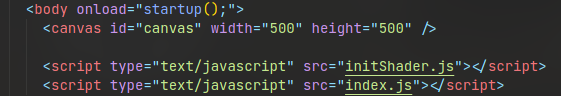
\includegraphics[width= \textwidth]{grafika/html.png}
    \caption{file html yang digunakan}
    \label{fig:html}
\end{figure}

seperti yang bisa dilihat dalam gambar \ref{fig:html}, file html ini akan berfungsi untuk mengatur ukuran dari canvas yang akan digunakan.
Canvas sendiri adalah tempat dimana webgl bisa melakukan manipulasi piksel secara bebas

selain itu, juga dilakukan import \emph{script initShader.js} dan \emph{index.js}.
\emph{initShader.js} digunakan untuk melakukan inisiasi Vertex Shader dan Fragment Shader.
sedangkan \emph{index.js} berisi program utama.



\section{initShader.js}

\begin{figure}[h]
    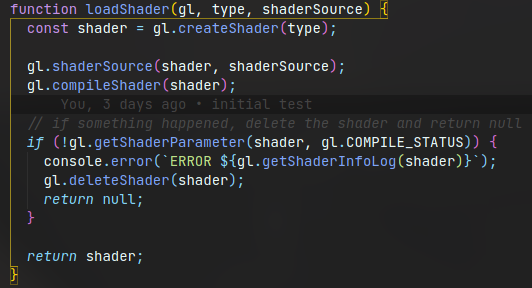
\includegraphics[width = \textwidth]{grafika/loadShader.png}
    \caption{fungsi \emph{loadShader} dalam \emph{initShader.js}}
    \label{fig: loadShader}
\end{figure}

fungsi dalam gambar \ref{fig: loadShader} digunakan untuk melakukan
kompilasi terhadap shader yang digunakan. Hasil dari kompilasi akan
digunakan untuk mengatur bagaimana sebuah vertex akan ditampilkan
di dalam canvas. Apabila dalam proses kompilasi terjadi error, maka
shader yang sudah dikompilasi tadi akan dihapus dan fungsi akan melakukan
return null.

\begin{figure}[h]
    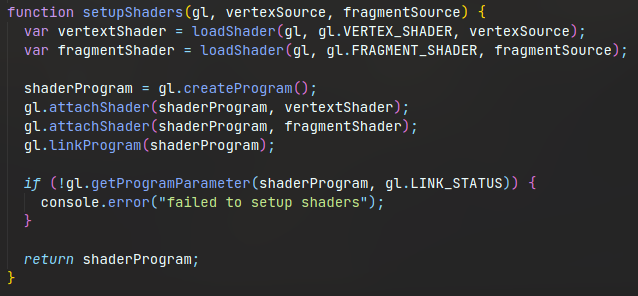
\includegraphics[width=\textwidth]{grafika/setupShader.png}
    \caption{fungsi setupShader dalam initShader.js}
    \label{fig: setupShader}
\end{figure}

setiap program webgl akan memerlukan vertex shader dan fragment shader.
program di gambar \ref{fig: setupShader} digunakan untuk menggabungkan
antara vertex shader dan fragment shader dan dengan menggunakan \emph{linkProgram} menghubungkan antara program
dengan shader yang sudah digabung tadi.



\section{index.js}

\begin{figure}[h]
    \centering
    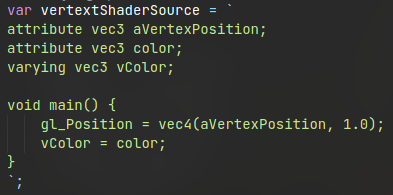
\includegraphics{grafika/vertexShader.png}
    \caption{vertexShader}
    \label{fig: vertexShader}
\end{figure}

yang pertama kali harus di set dalam program webgl adalah vertex shader dan fragment shader.
dalam vertex Shader, harus terdapat fungsi main, yaitu fungsi yang pertama kali akan dipanggil
oleh webgl. Selain itu, juga harus terdapat assign value ke gl\_Position yang akan digunakan oleh
webgl untuk mengetahui posisi piksel yang akan digambar.

hal lain yang harus dilihat adalah \emph{attribute} dan \emph{varying} yang terdapat dalam program vertex.
\emph{attribute} digunakan untuk menghubungkan antara program (dalam hal ini index.js) dengan shader. sedangkan
\emph{varying} digunakan untuk menghubungkan antara vertex Shader dengan fragment Shader. Terdapat satu lagi jenis variabel
yang tidak dipakai dalam shader ini adalah \emph{uniform}.

untuk saat ini, dalam vertex Shader kita hanya melakukan assign gl\_Position dan vColor.

\begin{figure}[h]
    \centering
    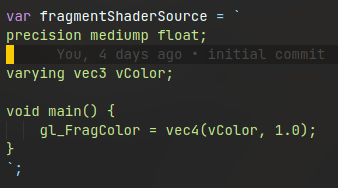
\includegraphics{grafika/fragment shader.png}
    \caption{fragmentShader}
    \label{fig: fragmentShader}
\end{figure}

fragment shader berguna untuk melakukan set bagaimana warna dari suatu vertex.
dalam gambar \ref{fig: fragmentShader}, kita hanya mengambil value yang di set di vertex Shader dan memasukkannya ke dalam gl\_FragColor.
gl\_FragColor digunakan oleh webgl dan harus ada dalam fragment Shader.


\begin{figure}[h]
    \centering
    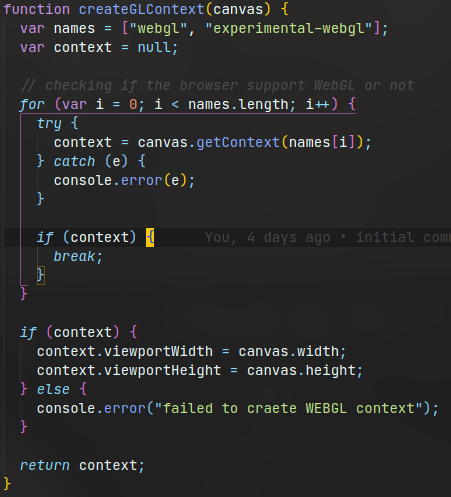
\includegraphics{grafika/createContext.png}
    \caption{fungsi createContext}
    \label{fig: createContext}
\end{figure}


